% !TEX root =  paper.tex
\section{Related Work}

\begin{figure*}[t]
	\begin{center}
		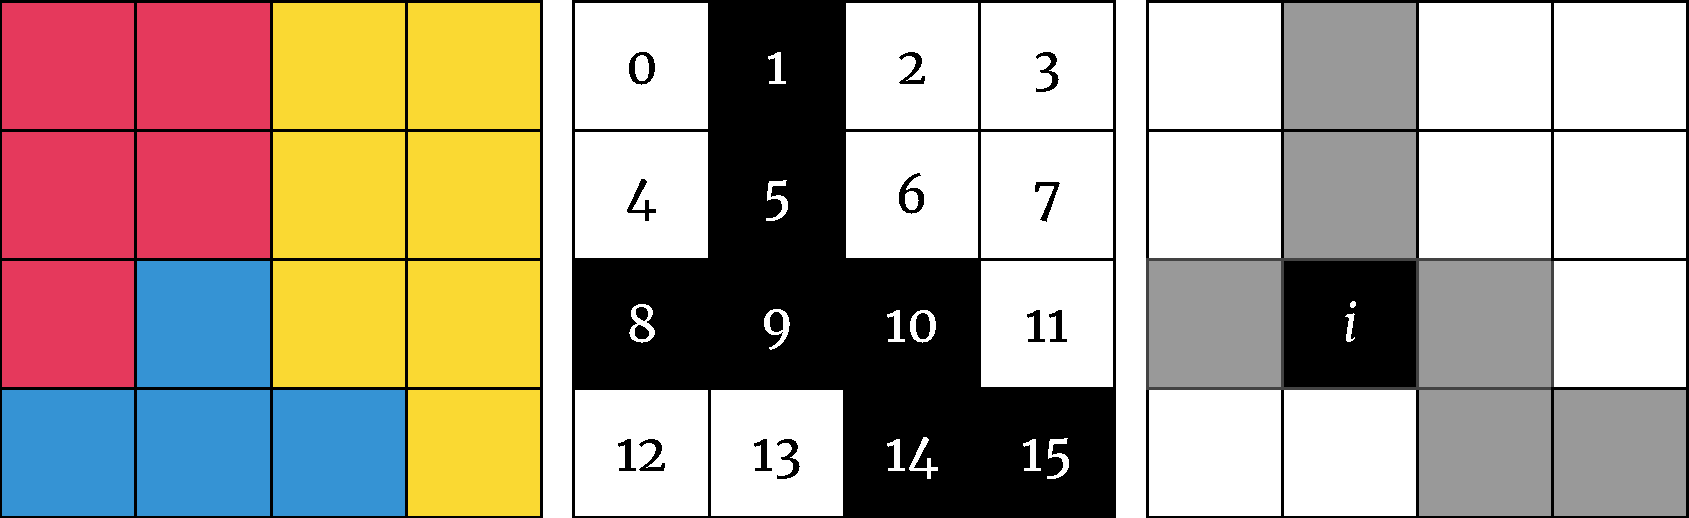
\includegraphics[width=0.45\linewidth]{./figures/encoding_diagram_opt.pdf}
		\hspace{0.08\linewidth}
		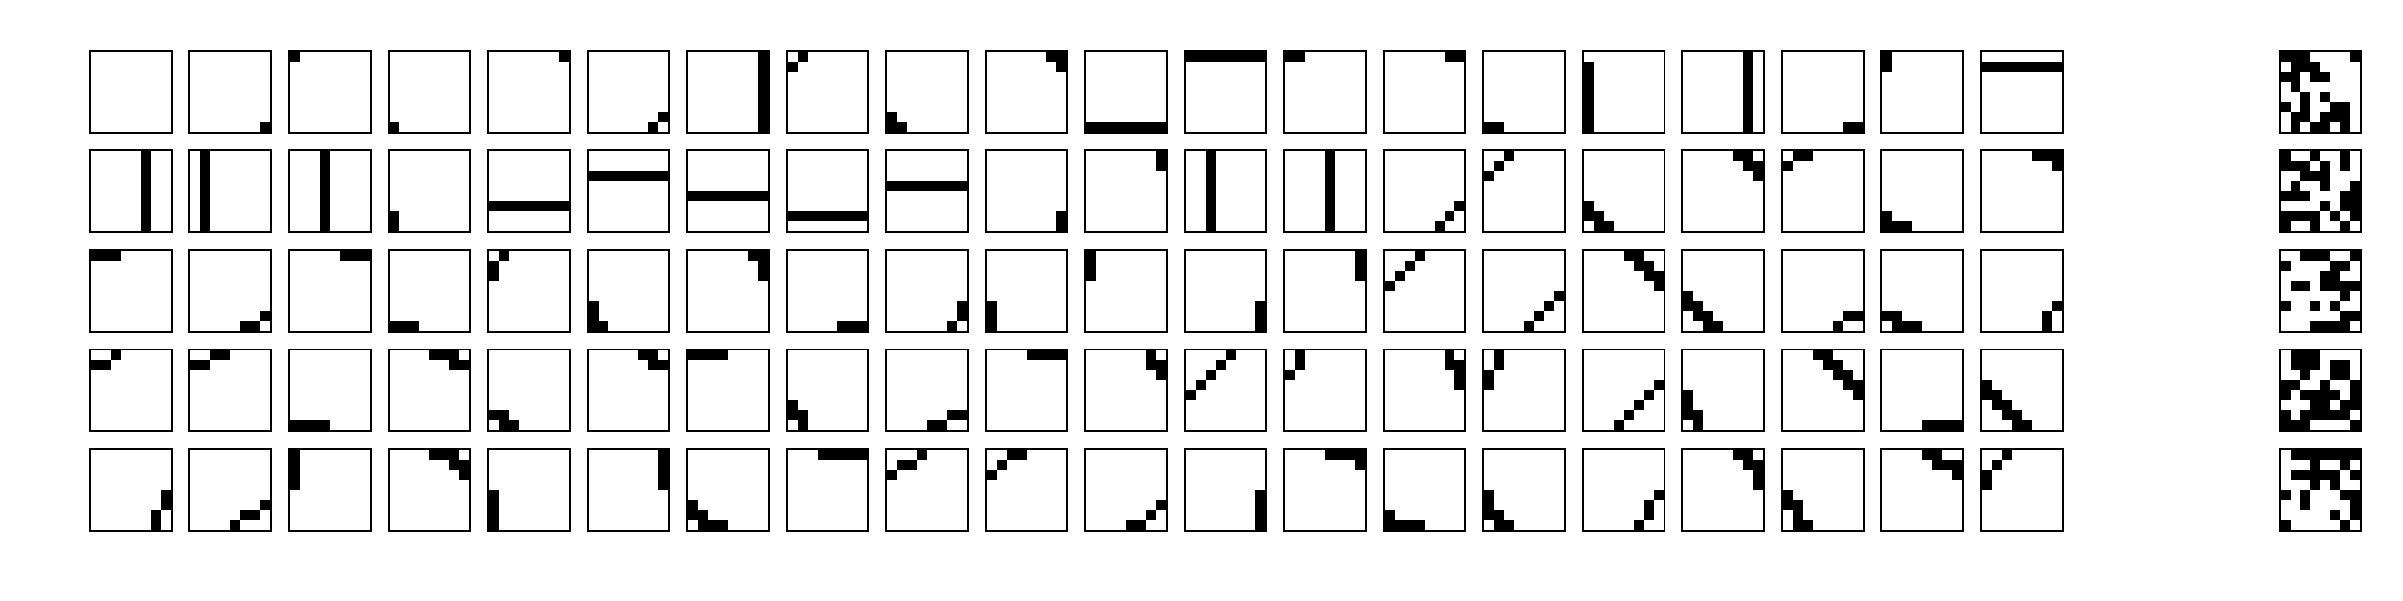
\includegraphics[width=0.45\linewidth]{./figures/window_values.pdf}
	\end{center}	
	\caption{Compresso works by dividing up the segmentation data into small blocks. On the left we show the intersection of three segments in a $4\times4\times1$ window. We extract a boundary map from this segmentation to transform the window into an integral value between $0$ and $2^{16} - 1$. The location $i$ requires some additional bookkeeping. On the right are the $100$ most common $8 \times 8 \times 1$ windows accounting for $\sim82\%$ of the volume on a representative dataset.}
	\label{fig:compression}
\end{figure*}

General-purpose compression schemes~\cite{collet2016smaller,deutsch1996zlib,google2016brotli,lehmann2016liblzf,oberhumer2005lzo,pavlov2007lzma,seward1998bzip2,vandevenne2016zopfli,welch1984technique,ziv1978compression} are not optimized for this data.
With Compresso, an algorithm published in MICCAI 2017, we exploit the typical characteristics of label volumes such as large invariant regions without natural relationship between label values. 
These properties render 2D image compression schemes inadequate since they rely on frequency reduction (using e.g., wavelet or discrete cosine transform) and value prediction of pixels based on local context (differential pulse-code modulation)~\cite{roelofs1999png,skodras2001jpeg}. 
Color space optimization strategies in video codecs~\cite{aimar2005x264} also have no effect on label volumes, even though the spatial properties of a segmentation stack (\textit{z}-axis) are similar to the temporal properties of video data (time-axis). 
A compression scheme designed specifically for label volumes is part of the visualization software Neuroglancer~\cite{google2016compressed}. 
This method exploits segmentation homogeneity by creating small blocks with $N$ labels and reducing local entropy to $\log_2{N}$ per pixel. 
Lookup tables then decode the values $[0,N)$ to the original 64-bit labels.

A significant amount of connectomics research considers the problem of extracting segmentation information at the voxel level of EM images.
First, intermediate representations like boundary, affinity or binary segmentation maps are generated from the voxels.
Random forests with hand-designed features~\cite{kaynig2015large}, or 2D and 3D convolutional networks produce boundary probabilities~\cite{bogovic2013learned,ciresan2012deep,jain2010boundary,seymour2016rhoananet,ronneberger2015u,amelio_segmentation}.
Often, the affinity between each voxel and its six neighbors are used~\cite{cciccek20163d,lee2015recursive,lee2017superhuman,parag2017anisotropic,turaga2010convolutional}. 
The 3D U-Net architecture has become popular~\cite{cciccek20163d} and the MALIS cost function is specifically designed to re-weight affinity predictions by their contribution to the segmentation error~\cite{briggman2009maximin}.
More recently, flood-filling networks~\cite{januszewski2016flood} produce binary segmentations from raw pixels with a recurrent convolutional network at a high computational cost.
Orthogonal to the representation, model averaging~\cite{zeng2017deepem3d} and data augmentation~\cite{lee2017superhuman} methods can further improve the performance, where Lee et al.~\cite{lee2017superhuman} surpass the estimated human accuracy on the SNEMI3D dataset.

Clustering techniques transform these intermediate representations into segmentations.
Some early methods apply computationally expensive graph partitioning algorithms with a single node per superpixel~\cite{andres2012globally}.
Several pixel-based approaches generate probabilities that neighboring pixels belong to the same neuron.
Often a watershed algorithm will then cluster these pixels into super-pixels~\cite{zlateski2015image}.

Region merging methods can be categorized by the similarity metric between adjacent segments and the merging strategy.
For the similarity metric, Lee et al. and Funke et al. rely solely on the accuracy of the predicted affinities and define the metric as the mean affinity between segments~\cite{funke2017deep,lee2017superhuman}.
Classification-based methods generate the probability to merge two segments from handcrafted~\cite{jain2011learning,seymour2016rhoananet,nunez2014graph,10.1371/journal.pone.0125825,parag2017anisotropic,zlateski2015image} and learned features~\cite{bogovic2013learned}. 
For the merging strategy, most methods use variants of hierarchical agglomeration ~\cite{seymour2016rhoananet,nunez2014graph,10.1371/journal.pone.0125825,parag2017anisotropic,zlateski2015image} to greedily merge a pair of regions at a time.
Jain et al. formulates the agglomeration problem as a reinforcement learning problem ~\cite{jain2011learning} and Pape et al. present a scalable multicut algorithm to partition superpixels with global optimization~\cite{beier2017multicut}.

Additional research builds on top of these region-based methods to correct errors in the segmentation. This can be done either using human proofreading~\cite{haehn2017guided,haehn2014design,mojo2} or automatically~\cite{rolnick2017morphological,error_correction_using_CNN}. 
In both cases, available methods are pixel-based and do not include global biological constraints into the decision making process. 
Our method can take as input any existing segmentation pipeline.

